\documentclass[numbers]{sigplanconf}

\usepackage[TS1,T1]{fontenc}

\usepackage{balance}
\usepackage[  obeyDraft,  colorinlistoftodos,]{todonotes}
\newcommand\todoauthor[2][\empty]{
  \expandafter\newcommand\csname #2\endcsname[2][\empty]{    \todo[color=#1,##1]{#2: ##2}}}
\def\todosec{\par\noindent\todo[inline]}
\def\secmissing{\par\noindent\todo[color=red,inline,size=\large]}
\long\def\todolist#1#2{\par\noindent\todo[inline,color={red!100!green!50},caption={#1}]{\begin{minipage}{\linewidth}\begin{itemize}
#2\end{itemize}
\end{minipage}
}}

% \let\OLDthebibliography\thebibliography
% \renewcommand\thebibliography[1]{
%   \OLDthebibliography{#1}
%   \setlength{\parskip}{4pt}
%   \setlength{\itemsep}{0pt plus 0.3ex}
% }


\usepackage{glossaries}
\usepackage{bcprules}
\usepackage{subcaption}
\usepackage{rotating}
\usepackage{longtable}

% \bcprulessavespacetrue
\bcprulestwocoltrue
\smallrulenamestrue
\usepackage{stmaryrd}
\usepackage{amssymb,amsmath}
\usepackage{tabularx}
\usepackage{xspace}
\xspaceaddexceptions{'$'$ |(}

\newcommand{\ac}[1]{\gls{#1}}
\newcommand{\Ac}[1]{\Gls{#1}}
\newcommand{\acp}[1]{\glspl{#1}}

\newacronym{api}{\textsc{api}}{application programming interface}
\newacronym{cip}{\textsc{cip}}{constraint-imperative programming}
\newacronym{ocp}{\textsc{ocp}}{object-constraint programming}
\newacronym{oo}{\textsc{oo}}{object-oriented}
\newacronym{dsl}{\textsc{dsl}}{domain-specific language}
\newacronym{frp}{\textsc{frp}}{functional reactive programming}
\newacronym{Frp}{\textsc{frp}}{Functional reactive programming}
\newacronym{vm}{\textsc{vm}}{virtual machine}
\newacronym{jit}{\textsc{jit}}{just-in-time}
\newacronym{ssa}{\textsc{ssa}}{static single assignment}
\newacronym{ccm}{\textit{ccm}}{constraint construction mode}
\newacronym{gui}{\textsc{gui}}{graphical user interface}

\newcommand{\hairspace}{\,}
\newcommand{\eg}{e.\hairspace{}g.,\xspace}
\newcommand{\Eg}{E.\hairspace{}g.,\xspace}
\newcommand{\Ie}{I.\hairspace{}e.,\xspace}
\newcommand{\ie}{i.\hairspace{}e.,\xspace}
\newcommand{\cf}[1]{cf.\,{#1}\xspace}

\usepackage[final]{listings}
\usepackage[font=bf,skip=\baselineskip]{caption}
\captionsetup[lstlisting]{font={small,tt}}

\lstdefinelanguage[80]{Smalltalk}{
  morekeywords={true,false,self,super,nil,thisContext},
  sensitive=true,
  morecomment=[s]{"}{"},
  morestring=[d]',
  style=SmalltalkStyle
}
\lstdefinestyle{SmalltalkStyle}{
  literate=        {^}{{\(\uparrow\)}}1
}

\usepackage[scale=.89,semibold]{sourcecodepro}
\usepackage[scale=.89,semibold,osf]{sourcesanspro}

\lstset{defaultdialect=[80]{Smalltalk}}

 \lstset{  basicstyle=\small\ttfamily,
  keywordstyle=\bfseries,
  commentstyle=\slshape,
  captionpos=b,
  showstringspaces=false,
  tabsize=2,
  resetmargins=true,
  frame=lines,
  language=ruby,
  floatplacement=hbtp,
  numbers=left,
  numbersep=5pt,
  numberstyle=\tiny\color{gray},
  xleftmargin=1em,
  columns=fullflexible,
  keepspaces=true,
  aboveskip=\bigskipamount,
  lineskip=-.5ex,
  escapechar=\`,
  float,
}

% Semantic rules
\newcommand{\maybe}{\textbf{\footnotesize{?}}\kern-1pt}


\newcommand{\Scope}{\ensuremath{\mathbb{S}}\xspace}
\newcommand{\Env}{\ensuremath{\mathbb{E}}\xspace}
\newcommand{\Cstore}{\ensuremath{\mathbb{C}}\xspace}
\newcommand{\Istore}{\ensuremath{\mathbb{I}}\xspace}
\newcommand{\Heap}{\ensuremath{\mathbb{H}}\xspace}
\newcommand{\Deref}{\texttt{\upshape H}\xspace}

\newcommand{\eval}[3]{\texttt{#1} $\vdash$ \texttt{#2} $\Downarrow$ \texttt{#3}}
\newcommand{\gstay}[3]{stay(\texttt{#1}, \texttt{#2}) $=$ \texttt{#3}}
\newcommand{\stayPrefix}[4]{stayPrefix(\texttt{#1}, \texttt{#2}, \texttt{#3}) $=$ \texttt{#4}}
\newcommand{\phase}[5]{solve(\texttt{#1}, \texttt{#2}, \texttt{#3}, \texttt{#4}) $=$ \texttt{#5}}
\newcommand{\stay}[2]{stay(\texttt{#1}) $=$ \texttt{#2}}
\newcommand{\istay}[2]{i-stay(\texttt{#1}) $=$ \texttt{#2}}
\newcommand{\toSolver}[2]{\texttt{E} $\vdash$ \texttt{#1} $\leadsto$ $#2$}
\newcommand{\fromSolver}[2]{$#1$ $\leadsto$ \texttt{#2}}
% \newcommand{\csolve}[2]{$#1$ $\models$ $#2$}
% \newcommand{\solve}[2]{\texttt{#1} $\models$ \texttt{#2}}
% \newcommand{\cfail}[1]{$\not\models$ $#1$}
% \newcommand{\fail}[1]{$\not\models$ \texttt{#1}}
\newcommand{\csolve}[2]{$#1$ $\models=$ $#2$}
\newcommand{\solve}[2]{\texttt{#1} $\models=$ \texttt{#2}}
\newcommand{\cfail}[1]{$\not\models=$ $#1$}
\newcommand{\fail}[1]{$\not\models=$ \texttt{#1}}
\newcommand{\step}[5]{\texttt{<#1|#2|#3>} $\longrightarrow$
  \texttt{<#4|#5>}}
\newcommand{\tc}[3]{\texttt{#1} $\vdash$ \texttt{#2} : \texttt{#3}}
\newcommand{\tcC}[2]{\texttt{#1} $\vdash$ \texttt{#2}}
\newcommand{\isArray}[2]{$isBasicCollection(\texttt{#1}) = \texttt{#2}$}

\newcommand{\evalH}[4]{\texttt{#1;#2} $\vdash$ \texttt{#3} $\Downarrow$ \texttt{#4}}
\newcommand{\solveH}[3]{\texttt{#1;#2} $\models$ \texttt{#3}}
% \newcommand{\solveH}[3]{\texttt{#1;#2} $\models_{E,H}$ \texttt{#3}}
% \newcommand{\solveH}[3]{\texttt{#1} $\models_{E,H}$ \texttt{#3}}
\newcommand{\failH}[1]{$\not\models_{E,H}$ \texttt{#1}}
\newcommand{\stepH}[9]{\texttt{<#1|#2|#3|#4|#5>} $\longrightarrow$
  \texttt{<#6|#7|#8|#9>}}
\newcommand{\tcH}[4]{\texttt{#1;#2} $\vdash$ \texttt{#3} {\upshape :} \texttt{#4}}
\newcommand{\tcHC}[3]{\texttt{#1;#2} $\vdash$ \texttt{#3}}
\newcommand{\toSolverH}[2]{\texttt{E,H} $\vdash$ \texttt{#1} $\leadsto$ $#2$}
\newcommand{\fromSolverH}[3]{$#1$ $\leadsto$ \texttt{#2,#3}}

\newcommand{\toSolverOO}[6]{\texttt{#1,#2} $\vdash$ \texttt{#3} $\leadsto$ \texttt{#4,#5} $\mid$ $#6$}

\newcommand{\inferrule}[3]{\infrule[#1]{\mbox{#2}}{\mbox{#3}}}
\newcommand{\inferax}[2]{\infax[#1]{\mbox{#2}}}

\newcommand{\judgment}[1]{\begin{flushleft} \fbox{#1}\end{flushleft}}

\newcommand{\receq}{\stackrel{\texttt{r}}{\texttt{=}}}

\newcommand{\lookup}[3]{\textit{lookup}(\texttt{#1},\texttt{#2}) = (\texttt{x$_1$} $\cdots$ \texttt{x$_n$},\texttt{#3})}


\newcommand{\combine}[4]{\texttt{#1;#2} $\vdash$ \texttt{#3} $\leadsto$ \texttt{#4}}
\newcommand{\inline}[9]{\texttt{<#1,#2,#3,#4,#5,#6>} $\leadsto$ \texttt{<#7,#8,#9>}}

\usepackage{tikz}
\newcommand\encircle[1]{%
  \tikz[baseline=(X.base)] 
    \node (X) [draw, shape=circle, inner sep=0] {\strut #1};}
% \newcommand{\ocollpred}{\raisebox{1pt}{\scriptsize\texttt{\encircle{P}}\xspace}}
% \newcommand{\ocollpred}{\ensuremath{\llbracket}\texttt{P}\ensuremath{\rrbracket}\xspace}
\newcommand{\ocollpred}{\raisebox{1pt}{\texttt{\textcircled{\scriptsize P}}}}

\newcommand{\inlineC}[9]{%
\def\argA{#1}\def\argB{#2}\def\argC{#3}\def\argD{#4}\def\argE{#5}%
\def\argF{#6}\def\argG{#7}\def\argH{#8}\def\argI{#9}%
\inlineCcontinued
}

\newcommand{\LeadsTo}{%
\kern0.3em\raisebox{-1.5pt}{$\leadsto$}\kern-1em\raisebox{1.5pt}{$\leadsto$}\kern0.3em}
% $\begin{smallmatrix}
% \leadsto\\
% \leadsto
% \end{smallmatrix}$}

\newcommand\inlineCcontinued[2]{%
  \texttt{<\argA,\argB,\argC,\argD,\argE,\argF>}\LeadsTo \texttt{<\argG,\argH,\argI,#1,#2>}}

\newcommand\enter[9]{%
\def\argA{#1}\def\argB{#2}\def\argC{#3}\def\argD{#4}\def\argE{#5}%
\def\argF{#6}\def\argG{#7}\def\argH{#8}\def\argI{#9}%
\entercontinued
}
\newcommand\entercontinued[2]{%
  \textit{enter}(\texttt{\argA},\texttt{\argB},\texttt{\argC},\texttt{\argD},\texttt{
    \argE},\texttt{\argF},\texttt{x$_1$} $\cdots$ \texttt{x$_n$},\texttt{e$_1$} $\cdots$
  \texttt{e$_n$}) = (\texttt{\argG},\texttt{\argH},\texttt{\argI},\texttt{#1},\texttt{#2})
}

\newcommand\stepHO[9]{%
\def\argA{#1}\def\argB{#2}\def\argC{#3}\def\argD{#4}\def\argE{#5}%
\def\argF{#6}\def\argG{#7}\def\argH{#8}\def\argI{#9}%
\stepHOcontinued
}
\newcommand{\stepHOcontinued}[2]{%
  \texttt{<\argA|\argB|\argC|\argD|\argE|\argF>} $\longrightarrow$ \texttt{<\argG|\argH|\argI|#1|#2>}}


\newcommand\evalBig[9]{%
\def\argA{#1}\def\argB{#2}\def\argC{#3}\def\argD{#4}\def\argE{#5}%
\def\argF{#6}\def\argG{#7}\def\argH{#8}\def\argI{#9}%
\evalBigcontinued
}
\newcommand{\evalBigcontinued}[2]{%
  \texttt{<\argA|\argB|\argC|\argD|\argE|\argF>} $\Downarrow$ \texttt{<\argG|\argH|\argI|#1|#2>}}

\newcommand{\resolve}[4]{\texttt{#3;#4} $\models_\texttt{#1}$ \texttt{#2}}
\newcommand{\reinline}[7]{\texttt{<#1,#2,#3,#4,#5>} $\leadsto$ \texttt{<#6,#7>}}

\newcommand{\solveConstraints}[9]{solve(\texttt{#1,#2,#3,#4,#5,#6,#7}) = \texttt{#8,#9}}


\usepackage{hyperref}
\def\sectionautorefname{Section}
\def\subsectionautorefname{Section}
\def\subsubsectionautorefname{Section}
\def\tableautorefname{Table}
\def\figureautorefname{Figure}

\hyphenation{Squeak/-Small-talk}
\hyphenation{Babelsberg}
\hyphenation{Babelsberg/S}
\sloppy

\renewcommand*\copyright{{%
  \usefont{TS1}{lmr}{m}{n}\textcopyright}}

% \def\sharedaffiliation{\end{tabular}
% \begin{tabular}{c}}
\begin{document}

\conferenceinfo{CROW '16}{March 15, 2016, Malaga, Spain}
\copyrightyear{2016}
\copyrightdata{978-1-nnnn-nnnn-n/yy/mm}
\copyrightdoi{nnnnnnn.nnnnnnn}

\publicationrights{licensed}

\title{Automatically Selecting and Optimizing Constraint Solver Procedures for Object-Constraint Languages}
% \subtitle{A Report on Solving Sudoku with Babelsberg/S for Squeak/Smalltalk}
% \numberofauthors{1}
% \author{
% \alignauthor
% Tim Felgentreff\({}^{\ast}\)\hspace{2em}Stefan Lehmann\({}^{\ast}\)\hspace{2em}Robert Hirschfeld\({}^{\ast}\)\\
% Sebastian Gerstenberg\({}^{\dagger}\)\hspace{1em}Jakob Reschke\({}^{\dagger}\)\hspace{1em}Lars R\"uckert\({}^{\dagger}\)\hspace{1em}Patrick Siegler\({}^{\dagger}\)\\
% Jan Graichen\({}^{\dagger}\)\hspace{1em}Christian Nicolai\({}^{\dagger}\)\hspace{1em}Malte Swart\({}^{\dagger}\)
% \sharedaffiliation
% \affaddr{Hasso Plattner Institute}\\
% \affaddr{University of Potsdam}\\
% \affaddr{Potsdam, Germany}\\
% \affaddr{\email{${}^\ast$\{firstname.lastname\}@hpi.uni-potsdam.de}}\\
% \affaddr{\email{${}^\dagger$\{firstname.lastname\}@student.hpi.uni-potsdam.de}}\\
% }

\authorinfo{Tim Felgentreff\({}^{\ast}\)\hspace{2em}Stefan Lehmann\({}^{\ast}\)\hspace{2em}Robert Hirschfeld\({}^{\ast}\)\\
  Sebastian Gerstenberg\({}^{\dagger}\)\hspace{1em}Jakob Reschke\({}^{\dagger}\)\hspace{1em}Lars R\"uckert\({}^{\dagger}\)\hspace{1em}Patrick Siegler\({}^{\dagger}\)\\
  Jan Graichen\({}^{\dagger}\)\hspace{1em}Christian Nicolai\({}^{\dagger}\)\hspace{1em}Malte Swart\({}^{\dagger}\)}
{Hasso Plattner Institute\\
  University of Potsdam\\
  Potsdam, Germany}
{${}^\ast$\{firstname.lastname\}@hpi.uni-potsdam.de\\
  ${}^\dagger$\{firstname.lastname\}@student.hpi.uni-potsdam.de}

\date{\today}

\maketitle
\begin{abstract}
  Object-constraint programming provides a design to integrate constraints with
  dynamic, object-oriented programming languages. It allows developers to encode
  multi-way constraints over objects and object collections using existing,
  object-oriented abstractions. These constraints are automatically maintained
  at run-time.

  One original goal of the Babelsberg-family of object-constraint programming
  languages was to allow users familiar with the imperative paradigm to quickly
  and efficiently make use of constraint solver capabilities. Yet, practical
  problems often require careful selection of solvers to find good solutions (or
  any at all). Furthermore, solver performance can vary and while most
  solvers come with various optimizations, developers have to have a good
  understanding of the solving process to use these optimizations
  effectively. This, however, is difficult to achieve if the solver is
  automatically selected by the system.

  In this work, we discuss three different implementations for automatic solver
  selection that we used in Babelsberg implementations. As a second step, we
  look at the performance potential of edit constraints that are available in
  some solvers such as Cassowary or DeltaBlue, and how they can be applied
  automatically to improve solver performance. We argue that these techniques
  make object-constraint programming more practical by improving the quality and
  performance of solutions.
\end{abstract}

\category{D.3.3}{Programming Languages}{Language Constructs and Features}[Constraints]

\keywords
Constraints, Incremental Re-solving, Object Constraint Programming, Constraint Imperative Programming, Babelsberg

\section{Introduction}
\label{sec:introduction}

Babelsberg~\cite{felgentreff2014jot} is a design to integrate constraints into
object-oriented languages in a way that allows programmers to dynamically create
and satisfy constraints on objects. The design is a strict extension of the
object-oriented semantics of the underlying host
language~\cite{FelgentreffOOPSLA2015}. Babelsberg uses object-oriented method
definitions to define constraints rather than a
\ac{dsl}~\cite{Squander,AppleCocoaAutoLayout}. As a consequence, constraint
expressions in Babelsberg respect encapsulation and can re-use object-oriented
abstractions. The design also supports solver features such as constraint
priorities~\cite{borning-lisp-symbolic-computation-1992} and incremental
resolving~\cite{freeman1990incremental}, and can use multiple cooperating
constraint solvers to search for solutions~\cite{felgentreff2014babelsbergjs}.

Examples for application domains where constraints can be particularly useful
are physical simulations and animation, load balancing, data structure repair,
and puzzle solving. For example, creating an imperative implementation of a
Sudoku game works well for the graphical parts and user interaction, that is,
for describing what should be displayed and what should happen when the user
provides input. But spelling out how even a naive Sudoku solver works in
object-oriented code still requires dozens of lines of code. Using the
Babelsberg design and constraints, however, allows the user to describe the
desired state that a valid Sudoku should have using ordinary objects and
imperative methods.

\phantomsection
\begin{lstlisting}[label=lst:sudoku]
always {
  sudoku.cells().all? { |c| 1 <= c && c <= 9 } &&
  sudoku.rows().all? { |r| r.all_different? } &&
  sudoku.columns().all? { |c| c.all_different? } &&
  sudoku.boxes().all? { |b| b.all_different? }
}
\end{lstlisting}
\phantomsection

Consider the above code listing. The predicates are valid Babelsberg code
(implemented on top of Ruby), and assert that all cells of a Sudoku must have
numbers between 1 and 9 and that all rows, columns, and 3x3 boxes in the Sudoku
must not contain duplicate numbers. The constraint is introduced using the
\verb!always:!  keyword, and uses ordinary object-oriented methods such as
\verb!all?!, \verb!all_different?!, or \verb!<=!. The Babelsberg design defines
how to translate these expressions into a form ready for consumption by a
constraint solver, and how the solution is fed back into the program state. This
frees the developer from writing or maintaining the code for the solving
itself. The only two conditions on constraint expressions are that they must
return a boolean and that they must be free of
side-effects~\cite{FelgentreffOOPSLA2015}.

An incomplete aspect of the original Babelsberg design was that it allowed
multiple constraint solvers to be used cooperatively to solve constraints, but
provided only minimal guidance to developers for deciding which solvers to
use. Users who were not familiar with the capabilities and limits of the various
available solvers often resorted to trial and error find a working combination
of solvers for a particular problem. Since it is in general much easier to state
constraints than to solve them, practical constraint solvers restrict themselves
to a useful subset of constraints in a particular domain for efficiency. This is
apparent in many popular solvers: the Cassowary
solver~\cite{badros2001cassowary} can efficiently solve multi-way linear
equations on floats using the simplex method; Z3~\cite{de2008z3} is an SMT can
numerically solve for reals, integers, booleans, as well as record data types;
Kodkod~\cite{torlak2007kodkod}, Z3, and Ilog~\cite{puget1994c++} can enumerate
solutions; and DeltaBlue~\cite{freeman-benson-phoenix-1989} can solve multi-way
constraints using local propagation.  An even more restricted approach is to
only consider one-way constraints that can compute an output value given new
inputs, but not vice versa
(\eg~\cite{hudson-uist-1996,myers-ieee-computer-1990}). These restrictions must
be considered when choosing solvers for a concrete set of constraints. In this
work we discuss three different implementations for automatic solver selection
that we used in the practical Babelsberg implementations.

Even if a working solver is found for a concrete set of constraints, it may not
be optimal in terms of performance. Although solving strategies such as
incremental re-solving~\cite{freeman1990incremental} and re-ordering of
constraint declarations can improve performance of some solvers and are
available in Babelsberg implementations~\cite{felgentreff2014jot}, these
optimizations have to be applied explicitly and are specific to particular
solvers. Furthermore, the Babelsberg semantics treats the solver as a black box,
and thus does not include a principled way of utilizing such
optimizations~\cite{FelgentreffOOPSLA2015}. In contrast, modern imperative
language runtimes apply a growing number of optimizations automatically in a
principled manner --- either at compile-time or using \gls{jit} compilation
techniques --- so that even unoptimized code provides good performance. To apply
these techniques to constraint solving, we look at the performance potential of
edit constraints in Babelsberg, and propose strategies to apply them
automatically to improve solver performance. The contributions of this work are:
\begin{itemize}
\item Three practical implementations for automatically selecting a constraint
  solver given a concrete set of constraints.
\item A novel application of \ac{jit}-compiler techniques to the Cassowary and
  DeltaBlue constraint solvers to improve solving performance transparently.
\end{itemize}

\section{Automatic Solver Selection}
\label{sec:autom-solv-select}

Given that multiple solvers can be used cooperatively with the Babelsberg
design, we need to figure out which solver to use for which constraint. Consider
again the Sudoku constraints from page 1% \pageref{lst:sudoku}
. These constraints are in
the domain integers, and use pairwise inequalities. To solve them requires a
constraint solver that can deal with inequalities over integers. Either the
developer or the system must decide which solver is capable of solving these
constraints and use it. In this section, we present different heuristics for
having the system select a solver automatically and present their trade-offs.

The solvers in the ThingLab~\cite{borning-toplas-1981} constraint programming
system as well as from the Kaleidoscope \acrlong{cip}
system~\cite{freeman-benson-iccl-1992} were automatically selected based on the
type of constraint that was handed to it. In these languages, however, the set
of available constraint solvers was fixed. More importantly, each solver had
capabilities that the others lacked, and thus many constraints could clearly
only be handled by one particular solver. The algorithm which determined how the
constraints were added to the solvers only had to check for these specific
capabilities of the solvers, and could be optimized easily. Such an algorithm is
not possible with the Babelsberg design, however, since we do not know in
advance which capabilities the solvers have, and the set of solvers can be
extended by the user. Even worse, we may want to use different solvers with
exactly the same capabilities, but that have different characteristics with
regards to performance or solution quality.

The simplest approach at assigning a constraint to a particular solver would be
to let the developer do it. Each constraint must then be annotated with the
correct solver to use in the source --- if the selection is incorrect (\ie
assigning the constraint to a solver which cannot solve it) or not ideal (\ie
using a general purpose problem solver when a specialized algorithm exists), the
system does not attempt to correct the problem. However, this simple approach is
undesirable. \Ac{ocp} is supposed to provide convenient access to constraint
solving for imperative programmers, thus it is inconvenient to expect each user
to have to learn about the capabilities and trade-offs between the different
solvers before using them. Instead, manual annotation should be the fallback if
the system is unable to select the ideal solver in a situation. This fallback is
available in all Babelsberg implementations, but the implementations use
different default strategies for selecting the solver if none is explicitly
specified.

\subsection{Eager Selection by Type}
This is the selection mechanism implemented in Babelsberg/R. For this algorithm,
the solvers in the system must extend appropriate classes to respond to a solver
selection message with an instance of themselves. If no solver was explicitly
selected, the \ac{vm} sends the \lstinline{for_constraint} message to each
variable value encountered during constraint construction. User code can add
solvers to the system by dynamically adding a \lstinline{for_constraint} method
to those classes for which the solver is applicable, making use of Ruby's open
classes. This method should return a solver-specific variable wrapper object
that implements a subset of the interfaces that the solver can reason about. For
example, the Cassowary solver extends the Float class:
\begin{lstlisting}
def for_constraint(name)
  v = Cassowary::Variable.new(name: name, value: self)
  Cassowary::SimplexSolver.instance.add_stay(v)
  v
end
\end{lstlisting}
This method creates a new variable, adds implicit, low-priority stay constraint
(to instruct the solver not to change the variable value unnecessarily, and
returns the solver-specific variable object. The \ac{vm}'s solver object then
sends messages to this object instead of the Float object in the context of the
constraint execution.

When executing a constraint expression, the system determines the most specific
dynamic types of each variable that it encounters. As long as no solver is
selected for the current constraint, the system sends a solver selection message
to the object to ask which constraint solver should be used for it. If the
object does not understand the message, this indicates that no solver declared
that it can handle this type of object. If the object responds with a solver,
the constraint is immediately assigned to that solver. Any further variables
that are encountered are now interpreted with this solver. If they happen to be
of a type that the solver can handle, they are normally represented as
variables. If they are not, their current value will be used as if it had been
annotated as read-only in the constraint expression. The solver will be able to
use the value of the variable but not write to it, but when the variable
changes, the updated value is passed to the solver.

If during the execution of the constraint expression no solver is
selected, the constraint is taken as-is: if it is already \verb!true!,
no further action must be taken. When any of the variables that
participate in the constraint change, the expression is re-executed
using this same algorithm. If the expression returns \verb!false! and
no solver is selected, it is treated as unsatisfiable. In either case,
a practical language should provide an appropriate warning to users,
informing them that no solver could be found for a constraint
involving the dynamic types that were encountered.

This selection algorithm is simple and fast. Constraints that deal
with few types can quickly be assigned to the correct solver. However,
the algorithm is brittle for constraints that include multiple types
that each should be handled by a different solver. Consider the
following example:
\begin{lstlisting}
s = "Hello"
n = 5
always { n == s.length() * 2 }
always { s.length() * 2 == n }
n = 10
\end{lstlisting}
Suppose we have a local propagation solver that can deal with
equalities over strings and numbers, but not arithmetic, and one that
can solver linear equations over reals, but does not support
strings. The two constraints in line 3 and 4 should be idempotent and
it should be irrelevant in which order they are defined or solved.

The first constraint will be handed to the linear arithmetic solver,
since we encounter the number \verb!n! first during \gls{ccm}. The
solver will treat the string as a constant, and is thus forced to use
the return value of the method \verb!s.length()! to update \verb!n! to
\verb!10!. The second constraint will be handed to the local
propagation solver, since we encounter the string \verb!s! first. The
constraint is already satisfied, so nothing needs to be done.

When we execute the assignment on line 5, the order in which the
solvers are called to solve these constraints matters. We must first
call the local propagation solver to update the string length. If we
call the linear arithmetic solver first, it will give up and treat the
constraint as unsatisfiable, since it cannot manipulate the string to
make it longer. This can lead to confusing cases where the system will
say a set of constraints is unsolvable, but a simple re-ordering of
operations in the constraint expressions will make it work.

\subsection{Selection by Preference}
This is the selection mechanism employed in Babelsberg/S~\cite{GraberREBLS2014}
and the original Babelsberg/JS
implementation~\cite{felgentreff2014babelsbergjs}. If the set of constraints
that two or more solvers can solve is not empty, it may be desirable to always
give preference to one solver over another, to avoid issues where the solver
surprisingly changes when a constraint expression is refactored. To assign
preferences, the system maintains a list of solvers implicitly ordered by
preference. This list may be generated or supplied by the user. In either case,
the list of solvers should be created early in the execution of the program and,
once the first constraint has been created, it should only be possible to
append, not remove or re-order solvers.

Instead of executing the constraint expression just once, it is executed in
\gls{ccm} once for each of the available solvers. The first solver that is able
to work with at least some of the variables that participate in the constraint
is selected and the constraint is assigned to it. Executing the constraint
expression multiple times is safe due to our requirement on it being free of
side-effects.

For the above example, suppose that the arithmetic solver is preferred
over the local propagation solver. In this case, both constraints will
be assigned to it. This means, however, that the assignment on line 5
now becomes unsatisfiable! While this may seem like a strong
restriction on the kinds of programs that can be written in this
manner, we consider it preferable over the potential surprise that the
two constraints above, even though they trivially express the same
equality, are assigned to different solvers. In this scenario, the
constraint system will always be unsatisfiable, regardless of how we
refactor the two constraint expressions. To make the program work, the
user should manually select the local propagation solver in this case,
or else re-order the solvers to give preference to the local
propagation solver at the beginning of the execution.

\subsection{Heuristic Selection}
\label{sec:heuristic-solv-select}

Babelsberg/JS now implements some heuristics for solver selection. If no
explicit solver was selected, the constraint is handed to multiple solvers in
parallel. In Babelsberg/JS, each solver can declare capabilities, such as which
types and operations it supports. Based on an initial analysis of the types and
operations encountered in the dynamic extent of the constraint expression,
solvers are filtered, and the remaining solvers all run to solve the
constraint. The solvers to finish without error are compared first for accuracy
of the result and then performance to select the final solver. Currently, no
further heuristics are implemented, but the order of the trade-off (performance
versus accuracy) can be swapped by the user.

The preferential solver selection presented before is already heuristic: it
selects the first solver that can work with at least some of the variables that
participate in the constraint. This heuristic is easily extended. An obvious
extension is to select the first solver that can deal with the \emph{most}
variables, and go by preference only in case of a tie. There are more such
extensions that make sense in this decision procedure. As described above, there
may be solvers that have exactly the same capabilities, and that only differ in
their performance or in the quality of their results.

Some of the solvers' properties, such as performance and the quality of the
result, can be determined automatically. For others, this solver selection
procedure requires solvers to come annotated with \emph{capabilities}, such as
the types and operations it supports, for which theories it is complete or
incomplete, or whether it supports finite as well as infinite domains.

A simple example, which the preferential selection can already decide, is a
constraint on two strings and the choice between a finite domain solver and an
local propagation solver:
\begin{lstlisting}
x = "Good Morning"
y = "G'day"
always { x = y }
\end{lstlisting}
We can tell from the types that the simplex solver will not be able to find a
solution to this constraint and that we should pick the local propagation
solver.

However, even a slightly more complex example may make our decision much more
difficult. Suppose we hand the following constraint over the reals to both a
simplex solver like Cassowary and a relaxation solver:
\begin{lstlisting}
a = 2.0
b = 2.0
always { a * a = b }
\end{lstlisting}
Again reject the simplex solver, this time because it is not equipped to deal
with non-linear equalities. The relaxation solver, on the other hand,
approximates a solution to this constraint by linearizing it, but it would be an
approximation only. More worrisome is that the solving algorithm can diverge, so
even if this constraint can be solved once, it may not be possible if we change
either \verb!a! or \verb!b! too much in one step. Suppose a relaxation solver
approximates the solution $a\mapsto 2.0$ and $b\mapsto 3.9999999999998$ for the
above constraint; because the relaxation method using numerical approximation,
it is prone to round-off errors. If we have a solver like Z3 available, we
might want to select it instead, both for higher precision, and because the
solving theory is more robust (albeit not complete) for non-linear arithmetic
over the reals. However, Z3 may pick another (valid) solution
$a\mapsto 1.4$ and $b\mapsto 1.96$. This solution means that the sum of the
changes to the variables is smaller than with the relaxation method, but for
some applications, we may prefer a solution which modifies the least number of
variables instead.

Our heuristic selection attempts to weigh these different criteria. As in the
selection by preference, we execute the constraint expression once for solver,
and in addition we let each solver solve the constraint once, but without
updating the environment and heap with the solution. Using the preference and
the below heuristics in conjunction, we can then select the best solver and add
the constraint to it. As constraints are added, we regularly re-evaluate the
metrics for existing constraints to check if they should be moved for better
performance or better results. Similarly, when a constraint becomes
unsatisfiable, but the current solver is annotated as being incomplete, we also
re-evaluate the metrics to search for another solver.

\paragraph*{Precision} As an example, Cassowary is complete for linear
equalities over reals, but its implementation uses float values to
represent reals, so a concrete solution may suffer from round-off
errors. Similarly, although the Z3 real theory works on reals of
arbitrary precision, these reals will be represented in many languages
as finite-precision floating point numbers, so again round-off errors
may occur. The precision of the results these solvers produce may thus
differ in practice, and could be considered as part of the solver
selection.

\paragraph*{Variable Changes} Another property that may impact the quality of
the solution is how the solver implementation affects the selection of solutions
when multiple solutions are available. Although stay constraints are part of the
semantics to ensure that any solution is close to the previous state of the
system, there are often multiple possible solutions that satisfy this
property. Which solution is selected is usually an artifact of the solver
implementation. However, problems such as the split-stay problem may make some
solutions still more desirable than others, and solvers which avoid it may be
preferable over those that do not. Similarly, solvers that change multiple
variables, but achieve a small squared distance from the previous state of the
system may be more or less suited to a particular problem than those that change
few variables, but those by a larger amount.

\paragraph*{Dimensionality} Besides the types of variables, the
operations on them and how they are connected also play a
role. Cassowary can only solve linear equations, while a relaxation
solver can find solutions for higher dimensional arithmetic. Thus, the
operations and associated operands within a constraint expression must
be considered to select the solver.

\paragraph*{Completeness} Another issue arises with incomplete
theories. SMT solvers, for example, require the different
partial solvers within to be convex for the decision procedure to be
complete. For example, the theory $(\mathbb{Z},+,=)$ (addition and
equality over the whole numbers) is convex, but $(\mathbb{Z},+,\leq)$
is not --- a constraint involving inequalities over the integers may
be satisfiable for a specific set of values, but another set of values
may make it simply too hard for the solver. In that event, another
solver (\eg using a form of relaxation) may be able to approximate a
solution and the constraint should be moved to that solver.

\paragraph*{Performance} Depending on the implementation, solvers may
differ significantly in both base performance and complexity in
required memory as well as time. As constraints are added during the
execution of a program, a solver that is fast for few constraints may,
due to higher complexity, become slower than a constraint with worse
base performance but better complexity. A selection algorithm can take
into account how fast a solver was able to satisfy a constraint, and
continues to monitor solvers to notice drops in performance when
constraints are added.\\

Each of these mechanisms has proven useful in practice to help developers not
familiar with constraint solvers to use constraints in Babelsberg. When they do
not work, however, the resulting confusion can impede development. Regardless of
the chosen strategy, we believe that communicating the strategy and how the
system arrived at a selection of solvers for a particular constraint is key to
making them useful.

\section{Fast Incremental Constraint Solving}
\label{sec:implementing-edit-constraints}
Performance of the solving algorithm itself is important for Babelsberg
languages. This is particularly apparent when few variables change with high
frequency and constraints have to re-satisfied in response, for example, when a
graphical object should follow the mouse cursor.

Not all constraint solvers are developed to provide good performance for
interactive applications, being used primarily for proofing or model
finding~\cite{de2008z3}. However, of the ones that are used interactively, some
solvers have explicit support for re-solving in case of state changes with good
performance. To that end, Freeman-Benson, Maloney, and Borning introduce the
notion of \emph{edit constraints} and incremental
re-satisfaction~\cite{freeman1990incremental}.  Their work is based on the
observation that user input is usually restricted to modify only small parts of
the constraint graph at a time, for example modifying 2d coordinates when moving
the mouse or modifying a string by entering one character at a time.

Both DeltaBlue and Cassowary treat stay and edit constraints specially, allowing
very fast incremental re-satisfaction of a collection of constraints as new edit
values stream into the system (and the weak stay constraints provide basic
stability). For DeltaBlue, this involves pre-calculating the execution plan from
the edit variables. For Cassowary, the Simplex tableau is set up so that it can
be efficiently re-optimized given new values for the edit
variables. Unfortunately, at least for Cassowary, preparing the solver for fast
incremental re-solving of a few variables requires some re-organization of the
tableau, and solving for other variables also becomes slower as a result. This
requires developers to anticipate whether a variable will only change more or
less often, and use the appropriate interface if they want to achieve the best
performance.

The \lstinline{edit} method provided as part of Babelsberg/R adds edit
constraints and repeatedly updates them with values from a stream running in a
separate thread. In Babelsberg/JS, to support edit constraints within a single
thread, the edit method returns a callback to input new values into the solvers,
rather than taking a stream of values. Babelsberg/S currently does not support
edit constraints.

Since the language design supports cooperating solvers, the solvers have to
provide a specific edit constraint \ac{api}\@. If a variable is added to an edit
constraint, but we dynamically discover that it is used in a solver which does
not support the edit constraint \ac{api}, a runtime exception is generated.
Upon calling the edit method, the following methods are called on the solvers
and the supplied variables, in order:
\begin{description}
\item[prepareEdit] is called on each solver variable. In this method, variables
  can prepare themselves for editing. In Cassowary, for example, this would call
  the \lstinline{addEditVar} method on the solver with the variable as
  argument. For DeltaBlue, this creates an \lstinline{EditConstraint} on the
  variable and adds it to the list of constraints.
\item[beginEdit] is called once for each solver participating in the edit before
  the callback is returned. In Cassowary, this initializes the edit constants
  array and prepares the solver for fast re-solving when these constants
  change. In DeltaBlue, the solver generates an execution plan to solve the
  constraints starting with the EditConstraints as input.
\item[resolveArray] is used to supply each solver with the new values and update
  the object's storage (so other observers and hooks around the values still
  work). Because the solver's execution plan is fixed for the duration of an
  edit, we disallow creating new edit callbacks before the current edit has
  finished. When new constraints are created, the execution plan may also become
  invalid, but we do not enforce invalidating the edit callback in this case.
\item[finishEdit] is sent to each solver variable when the edit stream ends or
  the callback is called without arguments. Cassowary variables do nothing here,
  DeltaBlue variables remove their EditConstraints from the solver.
\item[endEdit] is called once for each solver to reset the solver state.
\end{description}

To use, for example, Cassowary as the solver, all edit variables must be Floats
(\eg the x and y values of a point), but we also want to do this in an
object-oriented way that respects encapsulation. To support this, the client
passes an array of method names for the return values that should be updated in
the edit constraint (\eg \lstinline{x} and \lstinline{y} for a point --- those
values may be calculated or direct accessors).  The system creates fresh edit
variables, and adds an equality constraint to the return values of the
methods. Thus, the internal storage layout of the class is not visible to the
programmer from outside the object, because the equality constraint is simply
asserted on the results of message sends using the \lstinline{always} primitive.

In the following example, the mouse locations or the mouse point might store
their x and y values directly, or might be points represented using polar
coordinates.  In either case, the edit constraints apply to the return values of
their respective \lstinline{x} and \lstinline{y} methods:
\begin{lstlisting}
edit(stream: mouse.locations.each,
     accessors: [:x, :y]) { mouse_point }
\end{lstlisting}

In a DeltaBlue-specific edit method, the edit constraints returned could be
simpler, since DeltaBlue local propagation methods can apply to user-defined
objects such as points, not just to floats.  The point would be simply updated
rather than dealing with its x and y coordinates separately, and the data flow
plan would update the objects constrained to be equal to the point that
represents the mouse location.

\begin{figure*}
  \centering
  \begin{subfigure}[b]{0.497\textwidth}
    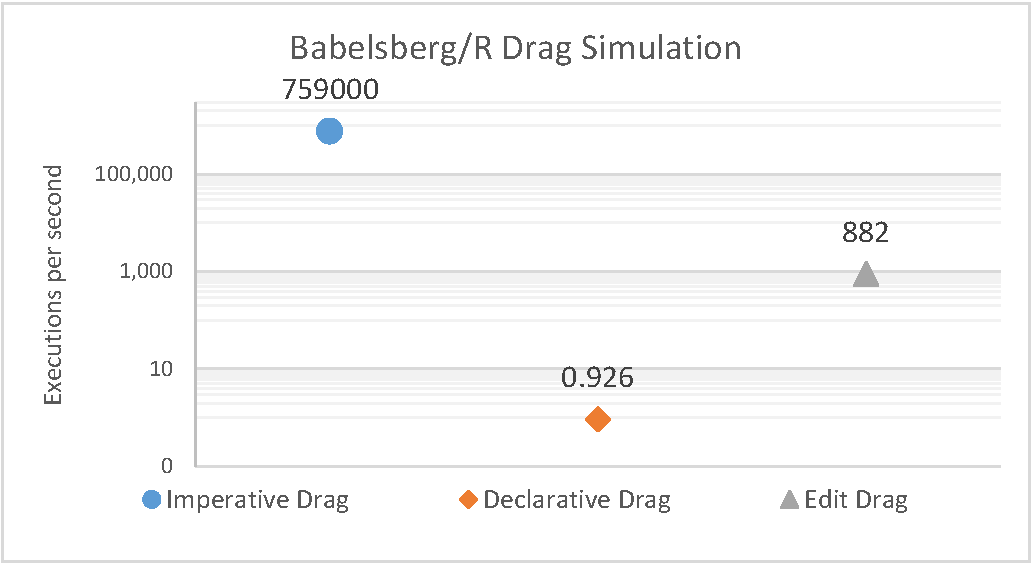
\includegraphics[width=\textwidth]{figures/r-edit}
    % \caption{Circuit Simulation}
  \end{subfigure}
  \begin{subfigure}[b]{0.497\textwidth}
    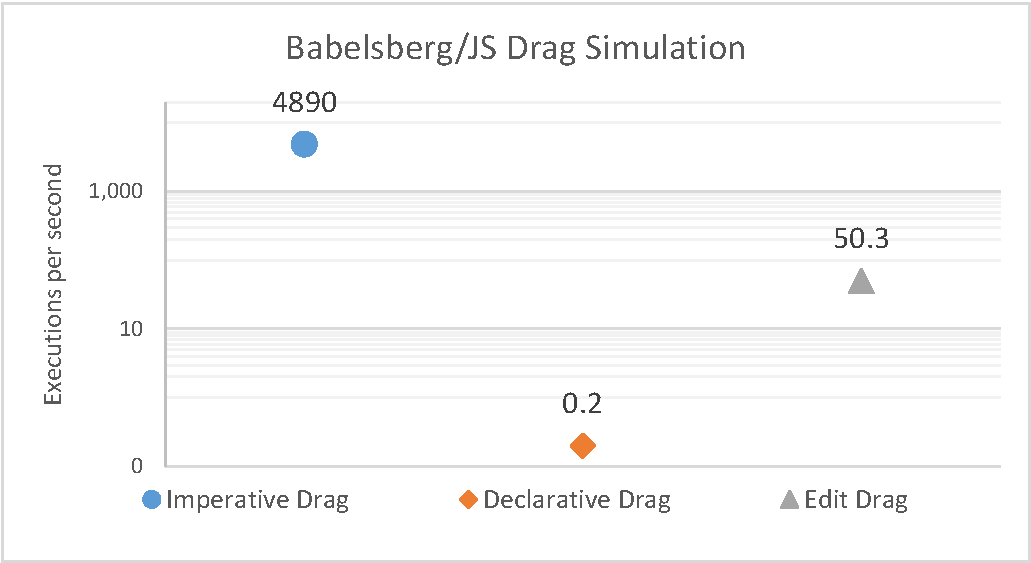
\includegraphics[width=\textwidth]{figures/js-edit}
    % \caption{Sudoku Solving}
  \end{subfigure}
  \caption{A comparison of constraint solving performance for hand-coded
    imperative solving, Babelsberg-style solving through assignment, and
    Babelsberg with edit constraints. Numbers show how many re-solving
    operations can be executed per second (more is better).}
  \label{fig:edit-bench}
\end{figure*}

\subsection*{Benchmark Results}
To quantify the impact of edit constraints, we used an example from
Kaleidoscope'93~\cite{lopez-oopsla-1994} and adapted it to our Babelsberg
implementations. In this example, the user drags the upper end of the mercury in
a thermometer using the mouse. However, the mercury cannot go outside the bounds
of the thermometer, even if the user tries to drag it out. Additionally, a gray
and white rectangle on the screen should be updated to reflect the new mercury
position, and a displayed number should reflect the integer value of the mercury
top. Refactoring the imperative version for Babelsberg makes it more general, so
the comparison is biased towards the imperative code. However, this example
demonstrates the performance impact if an imperative program is refactored with
the goal to make it more readable, not more general.

Note that the object-constraint version may be written in two ways: one that is
more like the imperative version and assigns new mouse locations in a loop; and
a more constraint-oriented version that declares \lstinline{mouse.location_y} as
an edit variable that triggers incrementally re-satisfying the constraints. The
latter is expected to be much faster, as Cassowary can just re-optimize a
previously optimal solution.

In this set of benchmarks we only include Babelsberg/R and Babelsberg/JS, since
we did not implement edit constraints in Babelsberg/S. The results are presented
in \autoref{fig:edit-bench}. The benchmarks were run on an otherwise idle Ubuntu
14.10 system using an Intel i5-2520M CPU forced to a constant clockspeed of 2.5
GHz with 16 GB of RAM. Benchmarks were run a varying amount of iterations (given
in the charts) depending on the benchmark, and each benchmark run was repeated
ten times, with the mean and standard deviation shown in the results where
appropriate.

For both implementations, the hand-coded imperative version is clearly the
fastest. However, it is also the longest, hardest to understand, and hardest to
prove correct. It is also clear that the purely declarative versions are
generally too slow to be used in an interactive application: in both cases, the
system could re-satisfy constraints less than once per second, which is not
enough to smoothly follow mouse movement and update the screen. Although using
edit constraints is still an two to three orders of magnitude slower than pure
imperative code, it is fast enough to re-satisfy constraints in an interactive
application and still provide smooth display updates.

\section{Automatic Edit Constraints}
We have shown in \autoref{sec:implementing-edit-constraints} that edit
constraints can significantly improve the performance of constraint solving and
in some cases make the use of constraint solving feasible in the first
place. However, using edit constraints directly requires developers to know
about them, understand where they are useful, and to adapt the source code to
create edit constraints.

\emph{Automatic edit constraints} (just like our integration of state and
object-oriented behavior with constraint declaration, or the architecture for
cooperating solvers and solver selection heuristics) support the goal of
Babelsberg to make constraints a useful tool for developers not familiar with
constraint solvers. Rather than requiring \ac{oo} developers to learn about
incremental solvers, in Babelsberg we have added heuristics for two solvers,
DeltaBlue and Cassowary, to recognize variables that change frequently and use
automatically apply incremental re-satisfaction to speed up solving.

The solving process of DeltaBlue when a variable is assigned involves creating a
new equality constraint, creating an execution plan, executing that plan to
solve the constraints, and finally to remove the equality constraint and the
associated plan. As a simple optimization heuristic, we can keep the last $n$
equality constraints and plans in a cache; if one of the $n$ variables changes
again, we can just update the equality constraint and re-use the execution plan,
rather than re-creating it.

For Cassowary, the simplex tableau has to be prepared for incremental
re-solving, and all variables that will be assigned have to be known
beforehand. This preparation is potentially slow, and it is not possible with
the implementation of the algorithm to keep multiple optimized versions of the
tableau around. Thus, the heuristic we use for Cassowary is more akin to a
\ac{jit}: for each variable known to Cassowary, we keep a counter that tracks
how often the variable has been assigned recently. In regular intervals, we
check which $n$ variables were assigned to most frequently, and optimize the
tableau for changes coming from those variables. At the same time, we ``decay''
the counters either by a fixed percentage or value. This ensures that variables
that have been assigned to a lot in the past, but not much in the recent history
of the program, are no longer considered for incremental re-satisfaction.

\subsection*{Benchmark Results}

We present two sets of benchmarks, one each for DeltaBlue and Cassowary, in
\autoref{fig:jit}. In our benchmarks, we measure a chain of variables that
should be equal to a fixed sum, a horizontal drag of a slider where only one
variable changes, a mouse drag where two variables changes alternate, a mouse
drag where one dimension changes more frequently than the other, and finally a
mouse drag where each dimension changes five times, and then the other changes
five times.

\begin{figure*}
  \centering
  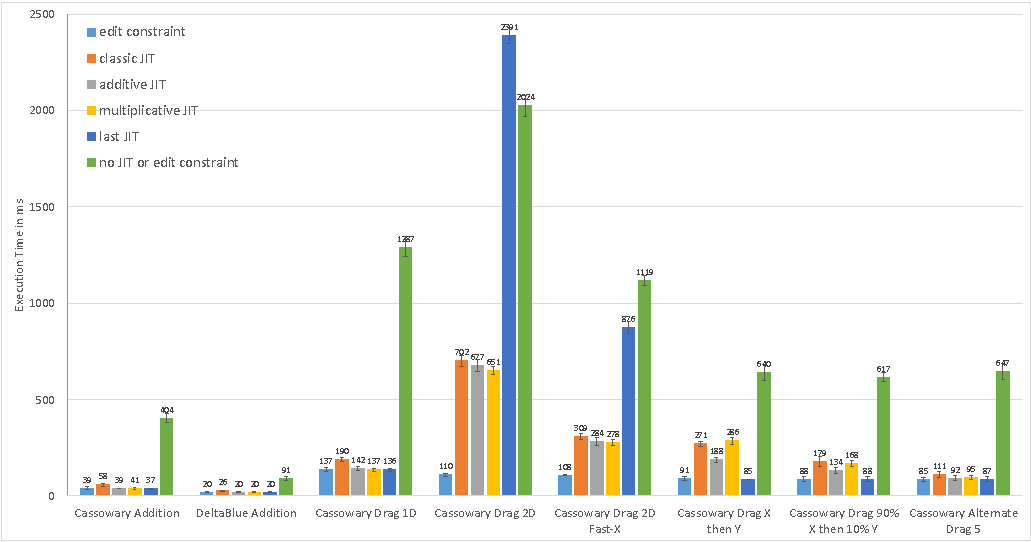
\includegraphics[width=\textwidth]{figures/jit}
  \caption{Combinations of benchmarks and automatic edit constraint
    \textsc{JIT}s. Graph shows execution time required for 500 solving
    operations (less is better).}
  \label{fig:jit}
\end{figure*}

For DeltaBlue, the best heuristic is to keep the last edit constraint, in a
strategy we call \emph{Last JIT}. At any time, if there is no current edit
constraint, we create one. If the current edit constraint is for another
variable, we throw the old one away and create the new one. This implementation
could easily be extended to cache the last $n$ edit constraints, rather than
just the last one. However, even as it is, we can see in our benchmark that this
heuristic is almost always as fast as writing edit constraints directly, and is
never slower than not using edit constraints.

For Cassowary, we include three heuristics with Babelsberg: the \emph{Classic
  JIT} strategy decays counters and changes or creates edit constraints in fixed
intervals. A second strategy, \emph{Additive Adaptive}, increments the interval
any time the most frequently used variable did not change, and decrements the
interval any time it did. Thus, when an edit constraint is well chosen and can
stay in effect for a long time, we reduce the overhead of checking and decaying
counters linearly with time. A third strategy, \emph{Multiplicative Adaptive},
modifies this behavior and, rather than incrementing or decrementing the
interval, it multiplies or divides the interval by two. This has the advantage
that we can avoid re-checks for longer periods of time if the edit constraint
stays in effect.

Our benchmarks show that all our heuristics are faster than using no edit
constraints at all. The adaptive strategies generally work better than the
\emph{Classic JIT} strategy, and by default we use the \emph{Additive Adaptive}
strategy, but the developer can select a different strategy manually.

\section{Related Work}
\label{sec:related-work}

There is some related work for automatic solver selection in other constraint
programming systems. Both Sketchpad~\cite{sutherland-ifips-1963} and
ThingLab~\cite{borning-toplas-1981} used the same three hard-wired solvers (a
relaxation solver, propagation of degrees of freedom, and local
propagation). However, since the list of solvers was fixed and their
capabilities have little overlap, the selection algorithm did not need to be
general. Similarly, the Kaleidoscope~\cite{lopez-oopsla-1994} and
Turtle~\cite{grabmuller2004turtle} \acrlong{cip} systems only had a fixed set of
low-level constraint solvers, and a fixed algorithm for calling user-defined
solving methods.

SMT solvers like Z3~\cite{de2008z3} include many different solving strategies
for different types of problems and use a standard algorithm to have these
strategies cooperate. However, most SMT solvers require manual selection of the
solving strategy if performance or solution quality is important and only use a
fixed, generic strategy based on type heuristics otherwise.

Lighthouse~\cite{SEPS15p66} is a system for selecting the fastest constraint
solver for a given problem. The system itself is designed to support different
heuristics and its general direction is thus similar to our heuristics-based
solver selection. However, Lighthouse is a separate tool to aid high-performance
computing application developers during development, whereas we propose at least
a limited form of automatic solver selection to be used at runtime.

We are not aware of work that applies just-in-time techniques to constraint
solvers, but there is a large body of work in scientific computing to pre-select
optimized sparse matrix kernels for use by linear solvers to optimize
performance in HPC systems such ATLAS~\cite{whaley2001automated},
OSKI~\cite{vuduc2005oski}, SALSA~\cite{demmel2005self}, and many more. The major
difference to our approach and goals are that these systems are all targeted
towards HPC applications. In these applications analysis and tuning may take a
long time (and is usually done before the actual computation). In Babelsberg, on
the other hand, recognizing the conditions for edit constraints and applying
them has to happen at runtime and is thus subject to the same issues as
traditional \ac{jit}s that must weigh the performance gain of an optimization
against the performance impact of analyzing and enabling it.

\section{Conclusions}
\label{sec:conclusions}

We have presented the different implementation approaches for automatic solver
selection used in the Babelsberg implementations and how they can aid imperative
developers employ constraint solving successfully. In addition, we have
presented a novel application of \ac{jit}-techniques to incremental re-solving
in the DeltaBlue and Cassowary constraint solvers which in many cases can offer
one order of magnitude performance improvements over a na\"ive formulation of
the constraints, and often comes close the performance of manually applied
edit constraints.

For the automatic selection, in practice we have found a mixture of manual and
eager selection to produce good results once the user has a basic understanding
of the available solvers and is aware of the eager selection process (in
particular, how seemingly idempotent refactorings may lead to different
results). We have found that while preferential selection avoids some surprising
behavior, this behavior occurs rarely in practice. The heuristic solver
selection procedure, although very powerful, has strong drawbacks: its
complexity impacts the performance of creating new constraints, and requires
constant re-checking. As with any heuristic, the results also depend on the
weight that is given to each of the metrics and may need to be adjusted
depending on the application domain. An educational advantage, however, is that
practical implementations can use the metrics to communicate to the user the
selection process and increase the user's understanding of the capabilities and
limits of available constraint solvers. As a guideline to implementers, we
suggest using the heuristic procedure as an educational tool and guiding
instrument at development-time, but revert to manual and eager selection when
many constraints are added dynamically throughout the run-time of the program,
to avoid the performance overhead of the selection procedure.

In future work, we plan to extend the heuristics in the practical
implementations and provide more principled criteria based on our practical
experience for using a specific selection strategy, and for weighing the
different heuristics against one another.

Regarding our automatic edit constraints, more work is required to determine
good heuristics for selecting the appropriate \ac{jit} strategy in many
cases. However, we argue that the work presented here is a good first step in
the direction of improving solver performance, and has applications outside of
the domain of object-constraint programming languages.

\bibliographystyle{abbrv}
\bibliography{constraints}
\balance

\end{document}

%%% Local Variables:
%%% mode: latex
%%% TeX-master: t
%%% End:
